\chapter{Konstruktivismus}
\label{cha:Konstruktivismus}
%Der Konstruktivismus in Reinform basiert auf Erkenntnissen der Neurobiologie bezüglich Erkennen und Erkenntnis. \cite[S. 14]{Siebert.1998}
Im Bereich des Konstruktivismus gibt es einige Varianten, welche sich alle auf gewisse Grundprinzipien berufen. So gehen alle Strömungen des Konstruktivismus davon aus, dass jedes Erkennen bzw. Wahrnehmen der Umwelt gefärbt ist, das heißt eine Interpretation der eigentlichen Wahrheit ist. Das Gehirn als das Organ in welchem der Lernprozess maßgeblich stattfindet reagiert nach konstruktivistischer Auffassung nur auf die Interpretation von Informationen, nicht aber auf Informationen selber. \cite{Reinmann.2013} 

Der Prozess des Lernens kann demnach nicht von außen induziert, sondern lediglich angeregt werden, und ist somit stets ein aktiver Prozess des Lernenden.  \cite{Reinmann.2013} 
Die Anregung veranlasst den Lernenden Wissen nach seiner eigenen Interpretation der Informationen und auf Basis seiner Erfahrungen selbst zu konstruieren, so dass Lernen immer eine individuelles Wissenskonstrukt auf Basis der gelernten Welt im Gehirn erschafft. \cite{Edelmann.2012} Das Aufbauen auf Erfahrung ist hierbei elementar, da davon ausgegangen wird, dass es keinen Zustand absoluten "Nicht-Wissens" - \emph{tabula rasa} - gibt. \cite{Anderson.1999}
%Dies führt dazu, dass nach konstruktivistischer Auffassung eine Didaktik des Lernanstoßes - eine sogenannte Ermöglichungsdidaktik - etabliert werden müsse. \cite[S. 482]{Arnold.2012}

\section{Vier Ausrichtungen des Konstruktivismus}
\label{sec:Konstr_4positions}

Nach \cite{Anderson.1999} gibt es vier verschiedene Ausprägungen des Konstruktivismus, welche nach zwei Dimensionen charakterisiert werden. (siehe Graphik \ref{fig:Anderson.1999_4positions})

Die erste Dimension, welche auf der Ordinatenachse in Graphik \ref{fig:Anderson.1999_4positions} aufgezeigt wird, beschreibt ob von einer subjektiven Sicht auf eine vieler Realitäten oder einer objektiven Sicht auf eine Realität ausgegangen wird. 
Der objektive Ansatz ist zu bevorzugen, wenn eine vorgegebene Realität näher und präziser vom Lernenden ergründet werden soll, wie in der Mathematik. Beim subjektiven Ansatz sollen die Fähigkeiten des Lernenden verbessert werden irgendeine Realität bezüglich eines bestimmten Themas zu erfassen. Dies wäre beispielsweise der Fall, wollte man die Möglichkeiten des Lernenden Religionen zu vergleichen verbessern. \cite{Anderson.1999}

Die zweite Dimension, festgehalten auf der Abszisse in Graphik \ref{fig:Anderson.1999_4positions}, stellt dar, ob soziale Faktoren das Lernprozess beeinflussen können oder sollen. Soziale Faktoren können kultureller Art sein oder sich auf die Lernumgebung beziehen. Sozio-linguistische Fähigkeiten werden in der Regel unter dem Einfluss sozialer Faktoren erlernt. Dem gegenüber steht das individuelle Lernen. \cite{Anderson.1999}

\begin{figure}
	\centering
	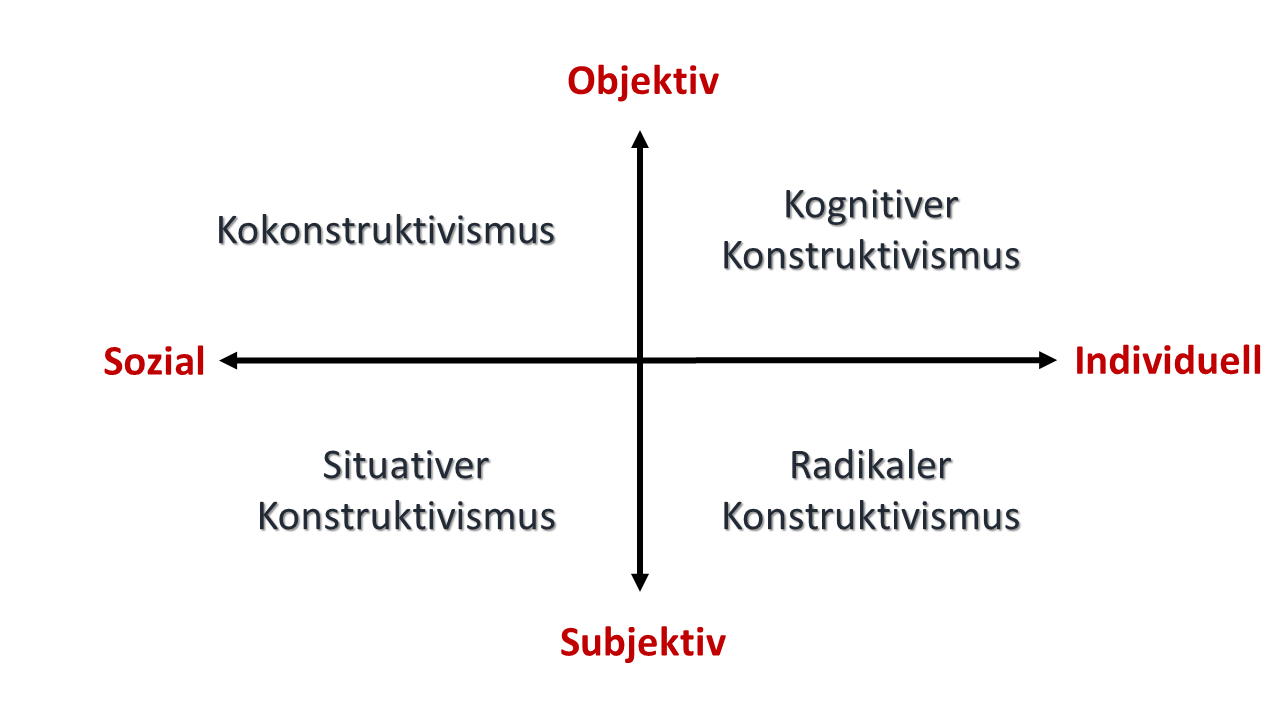
\includegraphics[width=1\textwidth]{Abbildungen/Anderson_1999_4positions.png}
	\caption{Die vier Ausrichtungen des Konstruktivismus nach \cite{Anderson.1999}.}
	\label{fig:Anderson.1999_4positions}
\end{figure}

Aus diesen zwei Dimensionen ergeben sich vier Ausrichtungen bzw. Ausprägungen des Konstruktivismus. 

Der \emph{Kognitive Konstruktivismus} zeichnet sich durch seine Betonung der Wichtigkeit von Konflikten und Unstimmigkeiten des konstruierten Wissens mit der tatsächlichen Realität für erfolgreiches Lernen aus. Nach \cite{Tobias.1991} sei es elementar, dass erworbenes und konstruiertes Wissen durch ständige Auseinandersetzung und Abgleich mit der Realität validiert und verbessert wird. 

Im Mittelpunkt des \emph{Radikalen Konstruktivismus} \label{par:konstr_pos_rad} steht die Auffassung welche auch \cite{Suchman.1987} teilt, dass keine gemeinsame Wahrnehmung aller Lernenden der Realität beim Lernen vorausgesetzt werden kann. Für eine Lernsituation in der von einem radikal konstruktivistischen Lernprozess ausgegangen wird, kann das Ergebnis des Lernens nicht mal im Ansatz vorausgesagt werden. Dies machte die Anregung zu Lernen durch den Lehrenden aber auch unmöglich, da er nicht weiß was seine Anregungen bewirken. \cite{Anderson.1999}

Genauso wie der Radikale Konstruktivismus geht auch der \emph{Situative Konstruktivismus} davon aus, dass es keine absolute Wahrheit gibt. \cite{Anderson.1999} Die beiden Ansätze unterscheiden sich aber dahingehend, dass dieser von einer sozialen Konstruktion von Wissen ausgeht. Das heißt, dass die Art und Weise, wie wir Dinge wahrnehmen darauf basiert, wie unser soziales Umfeld Dinge wahrnimmt. \cite{Jonassen.1992} %Beispielsweise nennt ein englischsprachig aufgewachsener Mensch einen Apfel "Apple" , da es das Umfeld genauso tut.

Der \emph{Kokonstruktivismus}, oder auch \emph{sozialer Konstruktivismus} genannt, geht auch wie der Situative Konstruktivismus davon aus, dass unser Umfeld beeinflusst, wie wir die Dinge wahrnehmen. Allerdings besteht der Unterschied darin, dass nach dem Kokonstruktivismus Diskussionen und soziale Interaktion zur Findung einer gemeinsamen Wahrheit führen. \cite{Bereiter.1994} Lernen in einem kokonstruktivistischen Lernprozess stellt den Lehrenden vor die Herausforderung, dass auch hier, ähnlich wie beim Radikalen Konstruktivismus (siehe \ref{par:konstr_pos_rad}), das Ergebnis des Lernen durch soziale Interaktion nicht eindeutig bestimmbar ist. \cite{Anderson.1999}
%\section{Ermöglichungsdidaktik}
%\label{sec:Ermoeglichungsdidaktik}

\section{Anwendung im E-Learning}
\label{sec:Konstr_Anwendungsfaelle}
Alex Koohang, Liz Riley und Terry Smith präsentieren in \cite[S. 95]{Koohang.2009} ein Modell zum Entwurf von E-Learnings, welches auf den Lernenden ausgerichtet ist. Begonnen wird ein solches E-Learning mit einer praktischen Problemsituation, welcher entweder vom Lehrenden oder angeregt durch diesen vom Lernenden entwickelt wird.
 
Unter Zuhilfenahme seiner Erfahrungen geht der Lernende die Problemsituation an und einen Lösungsvorschlag beziehungsweise eine Antwort. Dadurch wird gelernt. Die Ergebnisse werden in Gruppen und im Plenum diskutiert und bewertet. \cite[S. 95 f.]{Koohang.2009}

Diese Kollaboration kann durch ein E-Learning-System unterstützt werden. Auch möglicherweise benötigte Informationen können über eine E-Learning-Plattform zur Verfügung gestellt werden. \cite[S. 96]{Koohang.2009} Die Aufbereitung des Themas für die Mitlernenden kann zur besseren Verknüpfung mit Erfahrungen im Gehirn des Lernenden führen. \cite[S. 101 f.]{Koohang.2009}

Als konkretes Beispiel kann hierbei der Einsatz eines Wikis genannt werden. Dies ist eine webbasierte Anwendung, welche es den Nutzern ermöglicht Inhalte zu erstellen, ändern oder auch zu löschen. Der Vorteil hierbei besteht darin, dass der Wissensaustausch sowie die Erkenntnisgewinnung von und mit allen Teilnehmern des Wikis durchgeführt werden kann. Neben der Bearbeitung von Inhalten durch alle Nutzer, bieten viele Wikis die Möglichkeit der Verwendung einer Volltextsuche, sowie den Einsatz eines Versionierungsprotokollierung. Dies ermöglicht den transparenten Austausch sowie die Nachverfolgung von Änderungen von Inhalten. \cite[S. 75 f.]{Mertins.2009}

